% !TeX encoding = UTF-8
% !TeX program = latexmk
% !TeX spellcheck = en_US

\documentclass[degree=bachelor]{thuthesis}
  % 学位 degree:
  %   doctor | master | bachelor | postdoc
  % 学位类型 degree-type:
  %   academic(默认)| professional
  % 语言 language
  %   chinese(默认)| english
  % 字体库 fontset
  %   windows | mac | fandol | ubuntu
  % 建议终版使用 Windows 平台的字体编译


% 论文基本配置,加载宏包等全局配置
% !TeX root = ./thesis.tex

% 论文基本信息配置

\thusetup{
  %******************************
  % 注意:
  %   1. 配置里面不要出现空行
  %   2. 不需要的配置信息可以删除
  %   3. 建议先阅读文档中所有关于选项的说明
  %******************************
  %
  % 输出格式
  %   选择打印版(print)或用于提交的电子版(electronic),前者会插入空白页以便直接双面打印
  %
  output = print,
  %
  % 标题
  %   可使用“\\”命令手动控制换行
  %
  title  = {{基于 RISC-V 的用户态中断扩展}},
  title* = {RISC-V User-Interrupt},
  %
  % 学位
  %   1. 学术型
  %      - 中文
  %        需注明所属的学科门类,例如:
  %        哲学、经济学、法学、教育学、文学、历史学、理学、工学、农学、医学、
  %        军事学、管理学、艺术学
  %      - 英文
  %        博士:Doctor of Philosophy
  %        硕士:
  %          哲学、文学、历史学、法学、教育学、艺术学门类,公共管理学科
  %          填写“Master of Arts“,其它填写“Master of Science”
  %   2. 专业型
  %      直接填写专业学位的名称,例如:
  %      教育博士、工程硕士等
  %      Doctor of Education, Master of Engineering
  %   3. 本科生不需要填写
  %
  % degree-name  = {工学硕士},
  % degree-name* = {Master of Science},
  %
  % 培养单位
  %   填写所属院系的全名
  %
  department = {计算机科学与技术系},
  %
  % 学科
  %   1. 学术型学位
  %      获得一级学科授权的学科填写一级学科名称,其他填写二级学科名称
  %   2. 工程硕士
  %      工程领域名称
  %   3. 其他专业型学位
  %      不填写此项
  %   4. 本科生填写专业名称,第二学位论文需标注“(第二学位)”
  %
  discipline  = {计算机科学与技术},
  discipline* = {Computer Science and Technology},
  %
  % 姓名
  %
  author  = {田凯夫},
  author* = {Tian Kaifu},
  %
  % 指导教师
  %   中文姓名和职称之间以英文逗号“,”分开,下同
  %
  supervisor  = {陈渝, 副教授},
  supervisor* = {Professor Chen Yu},
  %
  % 副指导教师
  %
  % associate-supervisor  = {陈文光, 教授},
  % associate-supervisor* = {Professor Chen Wenguang},
  %
  % 联合指导教师
  %
  % co-supervisor  = {某某某, 教授},
  % co-supervisor* = {Professor Mou Moumou},
  %
  % 日期
  %   使用 ISO 格式;默认为当前时间
  %
  % date = {2019-07-07},
  %
  % 是否在中文封面后的空白页生成书脊(默认 false)
  %
  include-spine = false,
  %
  % 密级和年限
  %   秘密, 机密, 绝密
  %
  % secret-level = {秘密},
  % secret-year  = {10},
  %
  % 博士后专有部分
  %
  % clc                = {分类号},
  % udc                = {UDC},
  % id                 = {编号},
  % discipline-level-1 = {计算机科学与技术},  % 流动站(一级学科)名称
  % discipline-level-2 = {系统结构},          % 专业(二级学科)名称
  % start-date         = {2011-07-01},        % 研究工作起始时间
}

% 载入所需的宏包

% 定理类环境宏包
\usepackage{amsthm}
% 也可以使用 ntheorem
% \usepackage[amsmath,thmmarks,hyperref]{ntheorem}

\thusetup{
  %
  % 数学字体
  % math-style = GB,  % GB | ISO | TeX
  math-font  = xits,  % sitx | xits | libertinus
}

% 可以使用 nomencl 生成符号和缩略语说明
% \usepackage{nomencl}
% \makenomenclature

% 表格加脚注
\usepackage{threeparttable}

% 表格中支持跨行
\usepackage{multirow}

% 固定宽度的表格。
% \usepackage{tabularx}

% 跨页表格
\usepackage{longtable}

% 算法
\usepackage{algorithm}
\usepackage{algorithmic}

% 量和单位
\usepackage{siunitx}

% 参考文献使用 BibTeX + natbib 宏包
% 顺序编码制
\usepackage[sort]{natbib}
\bibliographystyle{thuthesis-numeric}

% 著者-出版年制
% \usepackage{natbib}
% \bibliographystyle{thuthesis-author-year}

% 本科生参考文献的著录格式
% \usepackage[sort]{natbib}
% \bibliographystyle{thuthesis-bachelor}

% 参考文献使用 BibLaTeX 宏包
% \usepackage[style=thuthesis-numeric]{biblatex}
% \usepackage[style=thuthesis-author-year]{biblatex}
% \usepackage[style=apa]{biblatex}
% \usepackage[style=mla-new]{biblatex}
% 声明 BibLaTeX 的数据库
% \addbibresource{ref/refs.bib}

% 定义所有的图片文件在 figures 子目录下
\graphicspath{{figures/}}

% 数学命令
\makeatletter
\newcommand\dif{%  % 微分符号
  \mathop{}\!%
  \ifthu@math@style@TeX
    d%
  \else
    \mathrm{d}%
  \fi
}
\makeatother

% hyperref 宏包在最后调用
\usepackage{hyperref}

% 代码块
\usepackage{listings}
\usepackage{xcolor}

\lstset{
    basicstyle=\tt,
    breaklines=true,
    extendedchars=false, %解决代码跨页时,章节标题,页眉等汉字不显示的问题
    %行号
    numbers=left,
    rulesepcolor=\color{red!20!green!20!blue!20},
    escapeinside=``,
    xleftmargin=2em,xrightmargin=2em, aboveskip=1em,
    %背景框
    framexleftmargin=1.5mm,
    frame=single,
    %背景色
    backgroundcolor=\color[RGB]{245,245,244},
    %样式
    keywordstyle=\color{blue}\bfseries,
    identifierstyle=\bf,
    numberstyle=\color[RGB]{0,192,192},
    commentstyle=\it\color[RGB]{96,96,96},
    stringstyle=\rmfamily\slshape\color[RGB]{128,0,0},
    %显示空格
    showstringspaces=false
}


\begin{document}

% 封面
\maketitle

% 学位论文指导小组、公开评阅人和答辩委员会名单
% 本科生不需要
% !TeX root = ../thuthesis-example.tex

\begin{committee}[name={学位论文指导小组、公开评阅人和答辩委员会名单}]

  \newcolumntype{C}[1]{@{}>{\centering\arraybackslash}p{#1}}

  \section*{指导小组名单}

  \begin{center}
    \begin{tabular}{C{3cm}C{3cm}C{9cm}@{}}
      李XX & 教授     & 清华大学 \\
      王XX & 副教授   & 清华大学 \\
      张XX & 助理教授 & 清华大学 \\
    \end{tabular}
  \end{center}


  \section*{公开评阅人名单}

  \begin{center}
    \begin{tabular}{C{3cm}C{3cm}C{9cm}@{}}
      刘XX & 教授   & 清华大学                    \\
      陈XX & 副教授 & XXXX大学                    \\
      杨XX & 研究员 & 中国XXXX科学院XXXXXXX研究所 \\
    \end{tabular}
  \end{center}


  \section*{答辩委员会名单}

  \begin{center}
    \begin{tabular}{C{2.75cm}C{2.98cm}C{4.63cm}C{4.63cm}@{}}
      主席 & 赵XX                  & 教授                    & 清华大学       \\
      委员 & 刘XX                  & 教授                    & 清华大学       \\
          & \multirow{2}{*}{杨XX} & \multirow{2}{*}{研究员} & 中国XXXX科学院 \\
          &                       &                         & XXXXXXX研究所  \\
          & 黄XX                  & 教授                    & XXXX大学       \\
          & 周XX                  & 副教授                  & XXXX大学       \\
      秘书 & 吴XX                  & 助理研究员              & 清华大学       \\
    \end{tabular}
  \end{center}

\end{committee}



% 也可以导入 Word 版转的 PDF 文件
% \begin{committee}[file=figures/committee.pdf]
% \end{committee}


% 使用授权的说明
\copyrightpage
% 将签字扫描后授权文件 scan-copyright.pdf 替换原始页面
% \copyrightpage[file=scan-copyright.pdf]

\frontmatter
% !TeX root = ../thesis.tex

\begin{abstract}
  
  进程间通信是进程间协调合作的基础,其效率往往影响着系统整体的工作效率。尤其在微内核架构中,进程间通信是主要的性能瓶颈之一。传统的进程间通信机制如信号、管道等大多数需要内核的参与,不可避免地引入了切换的开销。共享内存机制虽然减少了切换的开销,但同时也引入了同步互斥的开销,且通信双方无法实时响应消息,仍需要轮询或其他机制辅助。
  
  用户态中断是近年来提出的进程间通信机制,由用户态直接收发中断信号,可以减少陷入内核的开销,而且独立的中断处理流程可以支持异步通信,确保实时性的同时减少等待的开销。本文基于 RISC-V 指令集架构提出了用户态中断扩展方案,在硬件方面,修改 QEMU 模拟器验证设计方案并在 Rocket Chip 上实现该硬件扩展;在软件方面,修改 Linux 6.0 以适配硬件特性。最终在 FPGA 上搭建 SoC ,移植 Rocket Chip 并成功启动 Linux 。实验表明,用户态中断相比于信号机制,可以取得 203 倍的性能提升;相比于 eventfd,可以取得 136 倍的性能提升。

  \thusetup{
    keywords = {用户态中断, 软硬件结合, 进程间通信},
  }
\end{abstract}

\begin{abstract*}

  IPC (Inter-Process Communication) is the basis of inter-process coordination and cooperation, and its efficiency often affects the efficiency of the overall work of the system. Especially in microkernel, IPC is one of the main performance bottlenecks. Most of the traditional IPC mechanisms such as Signal and Pipe require the participation of the kernel, which inevitably introduces context switching overhead. Although the shared memory mechanism reduces the overhead of context switching, it also introduces the overhead of synchronous mutual exclusion, and the communication ends cannot respond to messages in real time, so polling or other mechanisms are still needed.
  
  User-Interrupt is an IPC mechanism proposed in recent years. Programs in user mode can directly send and receive interrupt signals, which can reduce the overhead of trapping into the kernel, and the independent interrupt handler can support asynchronous communication, ensuring real-time performance and reducing waiting overhead. This paper proposes a User-Interrupt extension based on the RISC-V instruction set architecture. In terms of hardware, the QEMU simulator is modified to verify the design and the hardware extension is implemented on Rocket Chip. In terms of software, Linux 6.0 is modified to adapt to hardware features. Finally we build SoC on FPGA with Rocket Chip and successfully boot Linux. Experiments show that compared with Signal, User-Interrupt can achieve 203x performance improvement; compared with eventfd, it can achieve 136x performance improvement.

  \thusetup{
    keywords* = {User-Interrupt, Hardware-Software Co-Design, IPC},
  }
\end{abstract*}


% 目录
\tableofcontents

% 插图和附表清单
% 本科生的插图索引和表格索引需要移至正文之后、参考文献前
% \listoffiguresandtables  % 插图和附表清单(仅限研究生)
\listoffigures           % 插图清单
\listoftables            % 附表清单

% 符号对照表
% !TeX root = ../thesis.tex

\begin{denotation}[3cm]
  \item[KPTI] {内核页表隔离 (Kernel Pagetable Isolation)}
  \item[IPC] {进程间通信 (Inter-Process Communication)}
  \item[UINTC] {用户态中断控制器 (User-Interrupt Controller)}
  \item[MMIO] {内存映射的输入/输出 (Memory-Mapped Input/Output)}  
  \item[PLIC] {平台级中断控制器 (Platform Level Interrupt Controller)}
  \item[CLINT] {核心本地中断器 (Core-Local Interruptor)}
  \item[IPI] {跨核中断 (Inter-Processor Interrupt)}
  \item[UIPI] {用户态跨核中断 {User Inter-Processor Interrupt}}
\end{denotation}



% 正文部分
\mainmatter
% !TeX root = ../thesis.tex

\chapter{引言}

传统的 IPC (Inter-Process Communication,进程间通信)机制包括信号、管道、命名管道 、消息队列和共享内存等\cite{modernos},其性能问题主要体现在以下几个方面:

\begin{itemize}
    \item[1.] 上下文切换开销:进程间通过内核进行通信,保存上下文和切换页表都会带来较大开销,为了解决熔断漏洞时引入的 KPTI 机制进一步增加了陷入内核的开销\cite{kpti};
    \item[2.] 数据拷贝开销:将数据块从一个进程复制到另一个进程的地址空间中,引入较高的延迟和开销;
    \item[3.] 同步互斥开销:使用锁和信号量等同步机制来保证进程之间访问共享资源的顺序,需要使用原子指令、内存屏障等硬件机制,会引入额外的开销;
    \item[4.] 安全性问题:进程和进程之间、内核和进程之间资源的共享都有可能在产生数据窃取和损坏等问题。
\end{itemize}

在微内核架构中,内核值提供最基本的服务,例如虚拟存储、IPC 等,大部分的系统服务如网络协议栈、文件系统、设备驱动等都以进程的形式运行在用户空间\cite{microkernel},IPC 因此成为了微内核中最重要的部分之一,同时也是性能瓶颈之一。

用户态中断(User-Interrupt)是由用户接收和响应的中断,相比于传统的 IPC 机制,用户态直接对中断进行处理可以减少陷入内核带来的开销。无论是在宏内核还是微内核中都具有良好的应用场景。用户态中断的发送方可以是下列中的任何一种:

\begin{itemize}
    \item 外部设备:用户态驱动\cite{userdriver}相比于内核的干预更加灵活和轻便,具有良好的可移植性和安全性。引入用户态中断后,用户态驱动可以直接接收并处理外部设备发来的中断,进一步提高性能。
    \item 内核:io\_uring \cite{iouring}是 Linux 5.1 版本引入的一种异步 I/O 机制,支持请求的批量提交、数据零拷贝,已被广泛应用于各种场景。引入用户态中断后,内核在 I/O 操作完成后可以跨核向进程发送用户态中断通知,进一步提高了异步唤醒的效率。
    \item 进程:seL4 的 Notification \cite{sel4}是一种轻量级的 IPC 机制,基于事件队列和快速路径,进程之间可以实现高效的异步通信,但目标进程需要通过轮询或等待的方式来处理信息。引入用户态中断后,目标进程可以在执行其他任务的同时立即接收并处理信息。
\end{itemize}

本文主要分为以下几个部分:

\begin{itemize}
    \item \textbf{背景介绍}:简要介绍 RISC-V N 扩展和 x86 用户态中断指令规范;
    \item \textbf{设计草案}: RISC-V 用户态中断扩展设计草案;
    \item \textbf{软件实现}:介绍在 QEMU 、Linux 等系统软件上关于 RISC-V 用户态中断扩展的实现细节;
    \item \textbf{硬件实现}:介绍在 Rocket Chip 上关于 RISC-V 用户态中断扩展的实现细节;
    \item \textbf{性能评估}:分别对软件实现和硬件实现进行性能测试和分析。
\end{itemize}
% !TeX root = ../thesis.tex

\chapter{背景介绍}

\section{RISC-V N 扩展}

RISC-V 是一种基于 RISC 原则的指令集架构,由加州大学伯克利分校开发,具有模块化、可扩展等特点。RISC-V N 扩展是在 RISC-V 特权级指令规范 v1.12 的草案中提出的,该扩展的设计思路是为 U 态提供一套和 M 态和 S 态类似的中断异常处理机制。截至目前,该扩展已被废除,因为 N 扩展的应用扩展尚不明朗且没有足够的工作去推动其完善和实现。为了引入用户态中断扩展,我们需要复现 RISC-V N 扩展的设计来支持基本的用户态中断处理流程。

\subsection{指令集规范}

\begin{table}
    \label{tab:rvn}
    \centering
    \begin{threeparttable}[c]
        \begin{tabular}{|l|l|}
            \hline
            名称 & 描述 \\
            \hline
            \Rustatus & U 态全局中断使能 \\
            \hline
            \Rutvec & U 态陷入向量模式与基址\\
            \hline
            \Ruip & U 态待处理中断(时钟中断、软件中断、外部中断) \\
            \hline
            \Ruie & U 态使能中断 (时钟中断、软件中断、外部中断)\\
            \hline
            \Ruscratch & U 态暂存寄存器 \\
            \hline
            \Ruepc & U 态中断或异常指令 pc \\
            \hline
            \Rucause & U 态陷入原因 \\
            \hline
            \Rsideleg & S 态中断委托 \\
            \hline
            \Rsedeleg & S 态异常委托 \\
            \hline
        \end{tabular}
        \caption{RISC-V N CSRs}
    \end{threeparttable}
\end{table}

RISC-V N 扩展中的 \Iuret 指令与 \Imret 和 \Isret 类似,将 \Rustatus 寄存器的 \FcsrUstatusUpie 赋值给 \FcsrUstatusUie ,然后跳转至 \Ruepc。

\subsection{外部中断}

尤予阳等人对 RISC-V N 扩展进行了进一步完善,在 PLIC 中为 U 态额外分配一套上下文,并将 PLIC 中断信号与 CPU 的 \FcsrUipUsip 寄存器连接。他们的工作主要分为两个方面,软件方面对 QEMU 进行修改来验证设计方案,基于 rCore 操作系统应用设计方案;硬件方面对 Rocket Chip 进行修改,并在 FPGA 上对设计方案进行了性能评估。通过将用户态中断应用在用户态串口驱动中,证明了其在吞吐率和延时方面的性能表现优于内核态驱动。

\section{x86 用户态中断}

2021 年 5 月发布的 Intel 指令集架构扩展 \cite{inteluintr} 中加入了基于 x86 指令集架构的用户态中断扩展。x86 的设计主要有以下几个特点:

\begin{itemize}
    \item[1.] 发送方和接收方状态在内存中进行维护;
    \item[2.] {\tt SENDUIPI} 指令需要经过两次读内存和一次写内存操作;
    \item[3.] 用户态中断有一套独立的控制流程,需要通过 MSR 辅助完成。
\end{itemize}

Linux 中加入了对 x86 用户态中断扩展的支持,并通过测试表明基于用户态中断的 IPC 机制相比于信号、eventfd 和管道等机制有明显的性能提升\cite{x86uintr}。

项晨东等人在 QEMU 加入了对 x86 用户态中断扩展的支持,成功运行了上述 Linux 分支并复现了性能测试结果。
% !TeX root = ../thesis.tex

\chapter{硬件实现}

\section{QEMU 模拟实现}

QEMU \cite{qemu} 为操作系统和用户态程序提供虚拟的执行环境,通过动态的二进制转换,模拟 CPU 的行为,同时支持多种外设的仿真,在系统开发中扮演着重要角色。
QEMU 支持模拟 RISC-V 运行环境,通过对 QEMU 的修改和测试,我们可以不断完善设计方案。对 QEMU 的修改主要分为四个方面:

\begin{itemize}
    \item 指令翻译:引入对 \Iuipi 指令的译码和执行;
    \item CPU 状态:维护 CSR 寄存器等 CPU 状态;
    \item 内存读写:\Iuipi 指令需要直接访问物理内存和 UINTC 外设,调用 \mintinline[breaklines]{C}{void cpu_physical_memory_rw(hwaddr addr, void *buf, hwaddr len, bool is_write)} 函数完成对物理地址的读写;
    \item 核间中断:实现 UINTC 并向各个核发送中断。
\end{itemize}

\subsection{指令翻译}

QEMU 翻译一条指令的过程为:从客户机指令(Guest Instructions)到中间码(TCG,Tiny Code Generator),最后再到宿主机指令(Host Instructions)。
QEMU 的翻译机制类似于 CPU 流水线中的译码阶段,需要定义模式串来帮助 QEMU 在执行到某一指令时调用对应的辅助函数。模式串的定义位于 target/riscv/insn32.decode :

\begin{lstlisting}
uipi_send       0000000  00000 ..... 010 ..... 1111011 @r2
uipi_read       0000001  00000 ..... 010 ..... 1111011 @r2
uipi_write      0000010  00000 ..... 010 ..... 1111011 @r2
uipi_activate   0000011  00000 ..... 010 ..... 1111011 @r2
uipi_deactivate 0000100  00000 ..... 010 ..... 1111011 @r2
\end{lstlisting}

以 \Iuret 这条指令为例,在 target/riscv/insn\_trans 目录下,有各种指令的翻译过程,主要用来将指令解析的结果(寄存器,立即数等)传递给辅助函数,将客户机指令拆解为宿主机指令来模拟目标指令的功能。
对于 \Iuret 指令的执行涉及到较多 CPU 状态的变化,会对 pc ,CSR 等产生影响, 辅助函数的定义位于 target/riscv/helper\.h,通过宏定义 DEF\_HELPER\_x 来声明辅助函数,例如:

\begin{lstlisting}[style=CStyle]
DEF_HELPER_1(uret, tl, env)
DEF_HELPER_4(csrrw, tl, env, int, tl, tl)
\end{lstlisting}

其中第一个参数对应辅助函数的名称 ,第二个参数代表函数的返回值类型(tl 表示 target\_ulong),后面的参数都是辅助函数传入的参数类型。有了以上的参考,我们可以定义其他辅助函数:

\begin{lstlisting}[style=CStyle]
DEF_HELPER_2(uipi_write, void, env, tl)
void helper_uipi_write(CPURISCVState *env, target_ulong src) {
    if (uipi_enabled(env, env->suirs)) {
        uint64_t addr = UINTC_REG_HIGH(env->suicfg, SUIRS_INDEX(env->suirs));
        cpu_physical_memory_write(addr, &src, 8);
    }
}
\end{lstlisting}

\subsection{CPU 状态维护}

CPU 状态的维护位于 target/riscv/cpu.h。这个结构同时考虑了 RV32、RV64、RV128 的情况,这些寄存器都是 CPU 运行时必要的状态。包括但不限于:

\begin{itemize}
    \item pc
    \item 整数、浮点寄存器堆
    \item CSR,有些寄存器是 M 态和 S 态复用的,例如 \Rmstatus、 \Rmip 等
    \item PMP 寄存器堆
    \item 通过 kernel\_addr、fdt\_addr 等从指定位置加载镜像
\end{itemize}

在target/riscv/cpu.h 文件末尾的表中注册 CSR 的操作函数。

中断异常、CSR 等宏定义位于 target/riscv/cpu\_bits.h ,我们需要在其中添加和 U 态有关的中断控制位。
CPU 中断异常处理函数位于 target/riscv/cpu\_helper.c 的最后,
这个函数对中断异常原因进行判断,并根据 CPU 当前的特权级做不同的处理。
这个函数只给出了 M 态和 S 态的中断异常处理,我们需要额外在此处加入委托给 U 态的中断异常处理,也就是读写 \Rustatus,\Rucause,\Ruepc 等寄存器。

\subsection{跨核中断实现}

QEMU 支持对不同硬件环境的模拟,需要在 virt 硬件环境中添加 UINTC 外设的配置并生成设备树信息。

UINTC 代码实现位于 hw/intc/riscv\_uintc.c ,调用 riscv\_uintc\_realize 对 UINTC 进行初始化,将 UINTC 外设连接到总线上,并初始化总线地址空间。对外设中的状态寄存器(接收方状态寄存器,中断信号寄存器等)进行内存分配和初始化。
通过调用 qdev\_connect\_gpio\_out 默认将 UINTC 的中断信号绑定至每个核的 \Ruip 寄存器中的 \FcsrUipUsip 位。

\begin{lstlisting}[style=CStyle]
for (i = 0; i < num_harts; i++) {
    CPUState *cpu = qemu_get_cpu(hartid_base + i);
    RISCVCPU *rvcpu = RISCV_CPU(cpu);
    qdev_connect_gpio_out(dev, i, qdev_get_gpio_in(DEVICE(rvcpu), IRQ_U_SOFT));
}
\end{lstlisting}

最后完成对 UINTC 读写函数的注册,这样就可以直接通过物理地址访问 UINTC 外设的读写端口:

\begin{lstlisting}[style=CStyle]
static const MemoryRegionOps riscv_uintc_ops = {
    .read = riscv_uintc_read,
    .write = riscv_uintc_write,
    .endianness = DEVICE_LITTLE_ENDIAN,
    .valid = {
        .min_access_size = 8,
        .max_access_size = 8
    }
};
\end{lstlisting}

在 QEMU 的 virt 硬件环境中添加设备树生成代码,生成的设备树节点内容如下:

\lstset{basicstyle=\footnotesize\tt}
\begin{lstlisting}
uintc@2f10000 {
    interrupts-extended = <0x08 0x00 0x06 0x00 0x04 0x00 0x02 0x00>;
    reg = <0x00 0x2f10000 0x00 0x4000>;
    interrupt-controller;
    compatible = "riscv,uintc0";
};
\end{lstlisting}

其中各个字段的含义为:

\begin{itemize}
    \item \textbf{interrupts-extended} 连接到每个核 \Ruip 寄存器的 \FcsrUipUsip 位;
    \item \textbf{interrupts-controller} 表示该设备是一个接收中断的控制器,这里加上是为了方便 Linux 识别,实际上 UINTC 并没有接收外部中断;
    \item \textbf{compatible} 表示设备名称,Linux 内注册驱动时应该与之对应。
\end{itemize}

在 UINTC 的实现中,中断是通过每次写入 UINTC 的端口来触发的,这和真实的硬件实现其实存在差异。
例如在 U 态,从目前的设计方案来看,需要同时满足以下几个条件才可以触发中断:

\begin{itemize}
    \item 当前特权级为 S 态;
    \item \Rustatus 中 \FcsrUstatusUie 位是 1;
    \item \Ruie 中 \FcsrUieUsie 位是 1;
    \item \Ruip 中 \FcsrUipUsip 位是 1。
\end{itemize}

在硬件实现中,可以看成是几个信号的与操作,当其他所有信号都拉高时,任何一个信号从低电平拉高都会触发中断,根据 RISC-V 的特权态规范\cite{rvpriv110},
\Isret 会将特权态从 S 态切换回 U 态,\Iuret 会将 \Rustatus 中的 \FcsrUstatusUie 位设置为 \FcsrUstatusUpie 位,在这两条指令后执行的第一条指令都有可能被中断打断并立刻进入中断处理的流程,
因此我们需要在 QEMU 中模拟这个过程,在 \Isret 和 \Iuret 指令中直接对上述条件进行判断和处理,例如在 \Isret 的辅助函数中:

\lstset{language=C}
\begin{lstlisting}[style=CStyle]
if (riscv_has_ext(env, RVN)
    && prev_priv == PRV_U
    && get_field(env->mip, MIP_USIP)
    && get_field(env->mstatus, MSTATUS_UIE)
    && get_field(env->sideleg, MIP_USIP)) {
    retpc = env->utvec;     // 直接跳转到U态中断处理入口
    env->uepc = env->sepc;  // 指定 \Iuret 到同一条指令
    mstatus = env->mstatus;
    mstatus = set_field(mstatus, MSTATUS_UPIE, 1);
    mstatus = set_field(mstatus, MSTATUS_UIE, 0);
    env->mstatus = mstatus;
}
\end{lstlisting}

\section{Rocket Chip 硬件实现}

\subsection{CPU 状态维护}

参考设计方案,在 rocket/CSR.scala 中添加读写 CSR 的逻辑,需要注意 \Ruip 等多个特权级共用的寄存器需要设置对应特权级的屏蔽位。

参考 M 态中断和异常委托的逻辑,添加 S 态委托到 U 态的逻辑,此外需要在 S 态将已委托给 U 态的中断屏蔽。

在 rocket/IDecode.scala 中添加 \Iuret 的指令解码并将指令解码注册到 \texttt{decode\_table} 中。\Iuret 的功能逻辑比较简单,只需要设置 \Rustatus 中的使能位并重新设置 pc 即可。

\begin{lstlisting}[style=CStyle,language=scala]
    // 读取 uip 寄存器
    val read_uip = read_mip & read_sideleg
    // 委托给 U 态的中断
    val delegateU = Bool(usingUser) && reg_mstatus.prv === PRV.U && delegate && read_sideleg(cause_lsbs) && cause(xLen - 1)
    // U 态的中断
    val u_interrupts = Mux(nmie && reg_mstatus.prv === PRV.U && reg_mstatus.uie, pending_interrupts & read_sideleg, UInt(0))
    // uret 的逻辑
    when (Bool(usingUser) && !io.rw.addr(9) && !io.rw.addr(8)) {
      reg_mstatus.uie := reg_mstatus.upie
      reg_mstatus.upie := true
      ret_prv := PRV.U
      io.evec := readEPC(reg_uepc)
    }
\end{lstlisting}

\subsection{UINTC 外设实现与接入}

参考 CLINT 和 PLIC 实现 UINTC 外设,首先定义 device 并指定名称和 compatible ,和 QEMU 中生成设备树的逻辑类似,在这里需要指定 UINTC 连接到 intc ,且需要指定为 interrupt-controller 让 linux 完成初始化。

\begin{lstlisting}[style=CStyle,language=scala]
    val device = new SimpleDevice("uintc", Seq("riscv,uintc0")) {
        override val alwaysExtended: Boolean = true
        override def describe(resources: ResourceBindings): Description = {
            val Description(name, mapping) = super.describe(resources)
            val extra = Map("interrupt-controller" -> Nil,
                "#interrupt-cells" -> Seq(ResourceInt(1)))
            Description(name, mapping ++ extra)
        }
    }
\end{lstlisting}

定义 node 并配置 UINTC 寄存器的读写端口,定义一系列的 \texttt{RegField} 实现读写操作,调用 \mintinline{scala}{node.regmap(opRegFields)} 进行注册:

\begin{lstlisting}[style=CStyle,language=scala]
    val node: TLRegisterNode = TLRegisterNode(
        address = Seq(params.address),
        device = device,
        beatBytes = beatBytes,
        concurrency = 1)

    // 注册 SEND 操作的写端口
    val opRegFields = uirs.zipWithIndex.flatMap { case (x, i) =>
      Seq(sendOffset(i) -> Seq(RegField(64, (),
        RegWriteFn { (valid, data) =>
            x.pending := x.pending | (valid << data(5, 0)).asUInt
            Bool(true)
        })))}
\end{lstlisting}

定义 \texttt{intnode} 连接到 CPU ,在上述 \texttt{SEND} 操作里将 \texttt{ipi} 寄存器对应位置位:

\begin{lstlisting}[style=CStyle,language=scala]
    val intnode: IntNexusNode = IntNexusNode(
        sourceFn = { _ => IntSourcePortParameters(Seq(IntSourceParameters(1,
            Seq(Resource(device, "int"))))) },
        sinkFn = { _ => IntSinkPortParameters(Seq(IntSinkParameters())) },
        outputRequiresInput = false)
    // 拉高 ipi 寄存器
    val ipi = Seq.fill(nHarts) { RegInit(0.U) }
    ipi.zipWithIndex.foreach { case (hart, i) =>
        hart := uirs.map(x => x.pending =/= 0.U && x.active && hartId(x.hartid) === i.asUInt).reduce(_ || _)
    }
    val (intnode_out, _) = intnode.out.unzip
    intnode_out.zipWithIndex.foreach { case (int, i) =>
        int(0) := ShiftRegister(ipi(i)(0), params.intStages) // usip
    }
\end{lstlisting}

将中断信号连接到对应核的 \FcsrUipUsip ,参考其他信号的处理方法,连接 \texttt{core.interrupts} 和 \texttt{intSinkNode}:

\begin{lstlisting}[style=CStyle,language=scala]
    // freechips.rocketchip.tile.SinksExternalInterrupts
    def csrIntMap: List[Int] = {
        // ...
        val usip = if (usingUser) Seq(0) else Nil
        List(65535, 3, 7, 11) ++ seip ++ usip ++ List.tabulate(nlips)(_ + 16)
    }
    // freechips.rocketchip.subsystem.CanAttachTile
    // 将 intSinkNode 的输入连接到 Rocket 处理器
    def decodeCoreInterrupts(core: TileInterrupts): Unit = {
        // ...
        val usip = if (core.usip.isDefined) Seq(core.usip.get) else Nil
        // ...
        val (interrupts, _) = intSinkNode.in(0)
        (async_ips ++ periph_ips ++ seip ++ usip ++ core_ips).zip(interrupts).foreach { case(c, i) => c := i }
    }
\end{lstlisting}

\subsection{UIPI 协处理器实现}

UIPI 协处理器负责处理自定义 \Iuipi 指令,基于 RoCC 实现,应用 RoCC 的访存端口处理 \Iuipi 指令涉及的访存请求。

RoCC 位于流水线的写回阶段,读写 CSR 时需要考虑写后读冲突,RoCC 读 \Rsuirs 和 \Rsuist 寄存器时需要增加前传逻辑。

\begin{lstlisting}[style=CStyle,language=scala]
    // 前传逻辑,以 suirs 寄存器为例
    when (decoded_addr(CSRs.suirs)) {
        val new_suirs = new SUIRS().fromBits(wdata)
        reg_suirs := new_suirs
        io.uintr.suirs := new_suirs
    }.otherwise {
        io.uintr.suirs := reg_suirs
    }
\end{lstlisting}

根据 Rocket Chip 的配置方法,在 Tile 中添加 UIPI 协处理器:

\begin{lstlisting}[style=CStyle,language=scala]
    class WithUIPI extends Config((_, _, _) => {
        case BuildRoCC => Seq((p: Parameters) => {
            // 指定该 RoCC 处理符合 OpcodeSet.custom3 格式的指令
            val module = LazyModule(new UIPI(OpcodeSet.custom3)(p))
            module
        })
    })
\end{lstlisting}

UIPI 协处理器接收译码结果并根据操作码来执行不同处理流程,状态机各个状态描述如下:

\begin{itemize}
    \item \texttt{\textbf{s\_idle}} 默认状态,等待接收处理器传来的操作请求;
    \item \texttt{\textbf{s\_wait\_mem0}} \Iuipisend 指令发起读内存请求并等待响应;
    \item \texttt{\textbf{s\_read\_uist}} \Iuipisend 指令处理响应并根据返回数据计算出访问 UINTC 的地址,根据数据缓存的 \texttt{s2\_nack} 信号判断是否需要重新发起请求;
    \item \texttt{\textbf{s\_wait\_mem1}} 发起读或写 UINTC 请求并等待响应;
    \item \texttt{\textbf{s\_check\_nack0}} 等待数据缓存响应;
    \item \texttt{\textbf{s\_check\_nack1}} 根据数据缓存的 \texttt{s2\_nack} 信号判断是否需要重新发起请求;
    \item \texttt{\textbf{s\_resp}} 响应处理器请求,\Iuipiread 需要返回写入目标寄存器的内容;
    \item \texttt{\textbf{s\_error}} 指令格式错误、访存错误、权限错误、发送方状态表项错误。
\end{itemize}

\begin{figure}
    \centering
    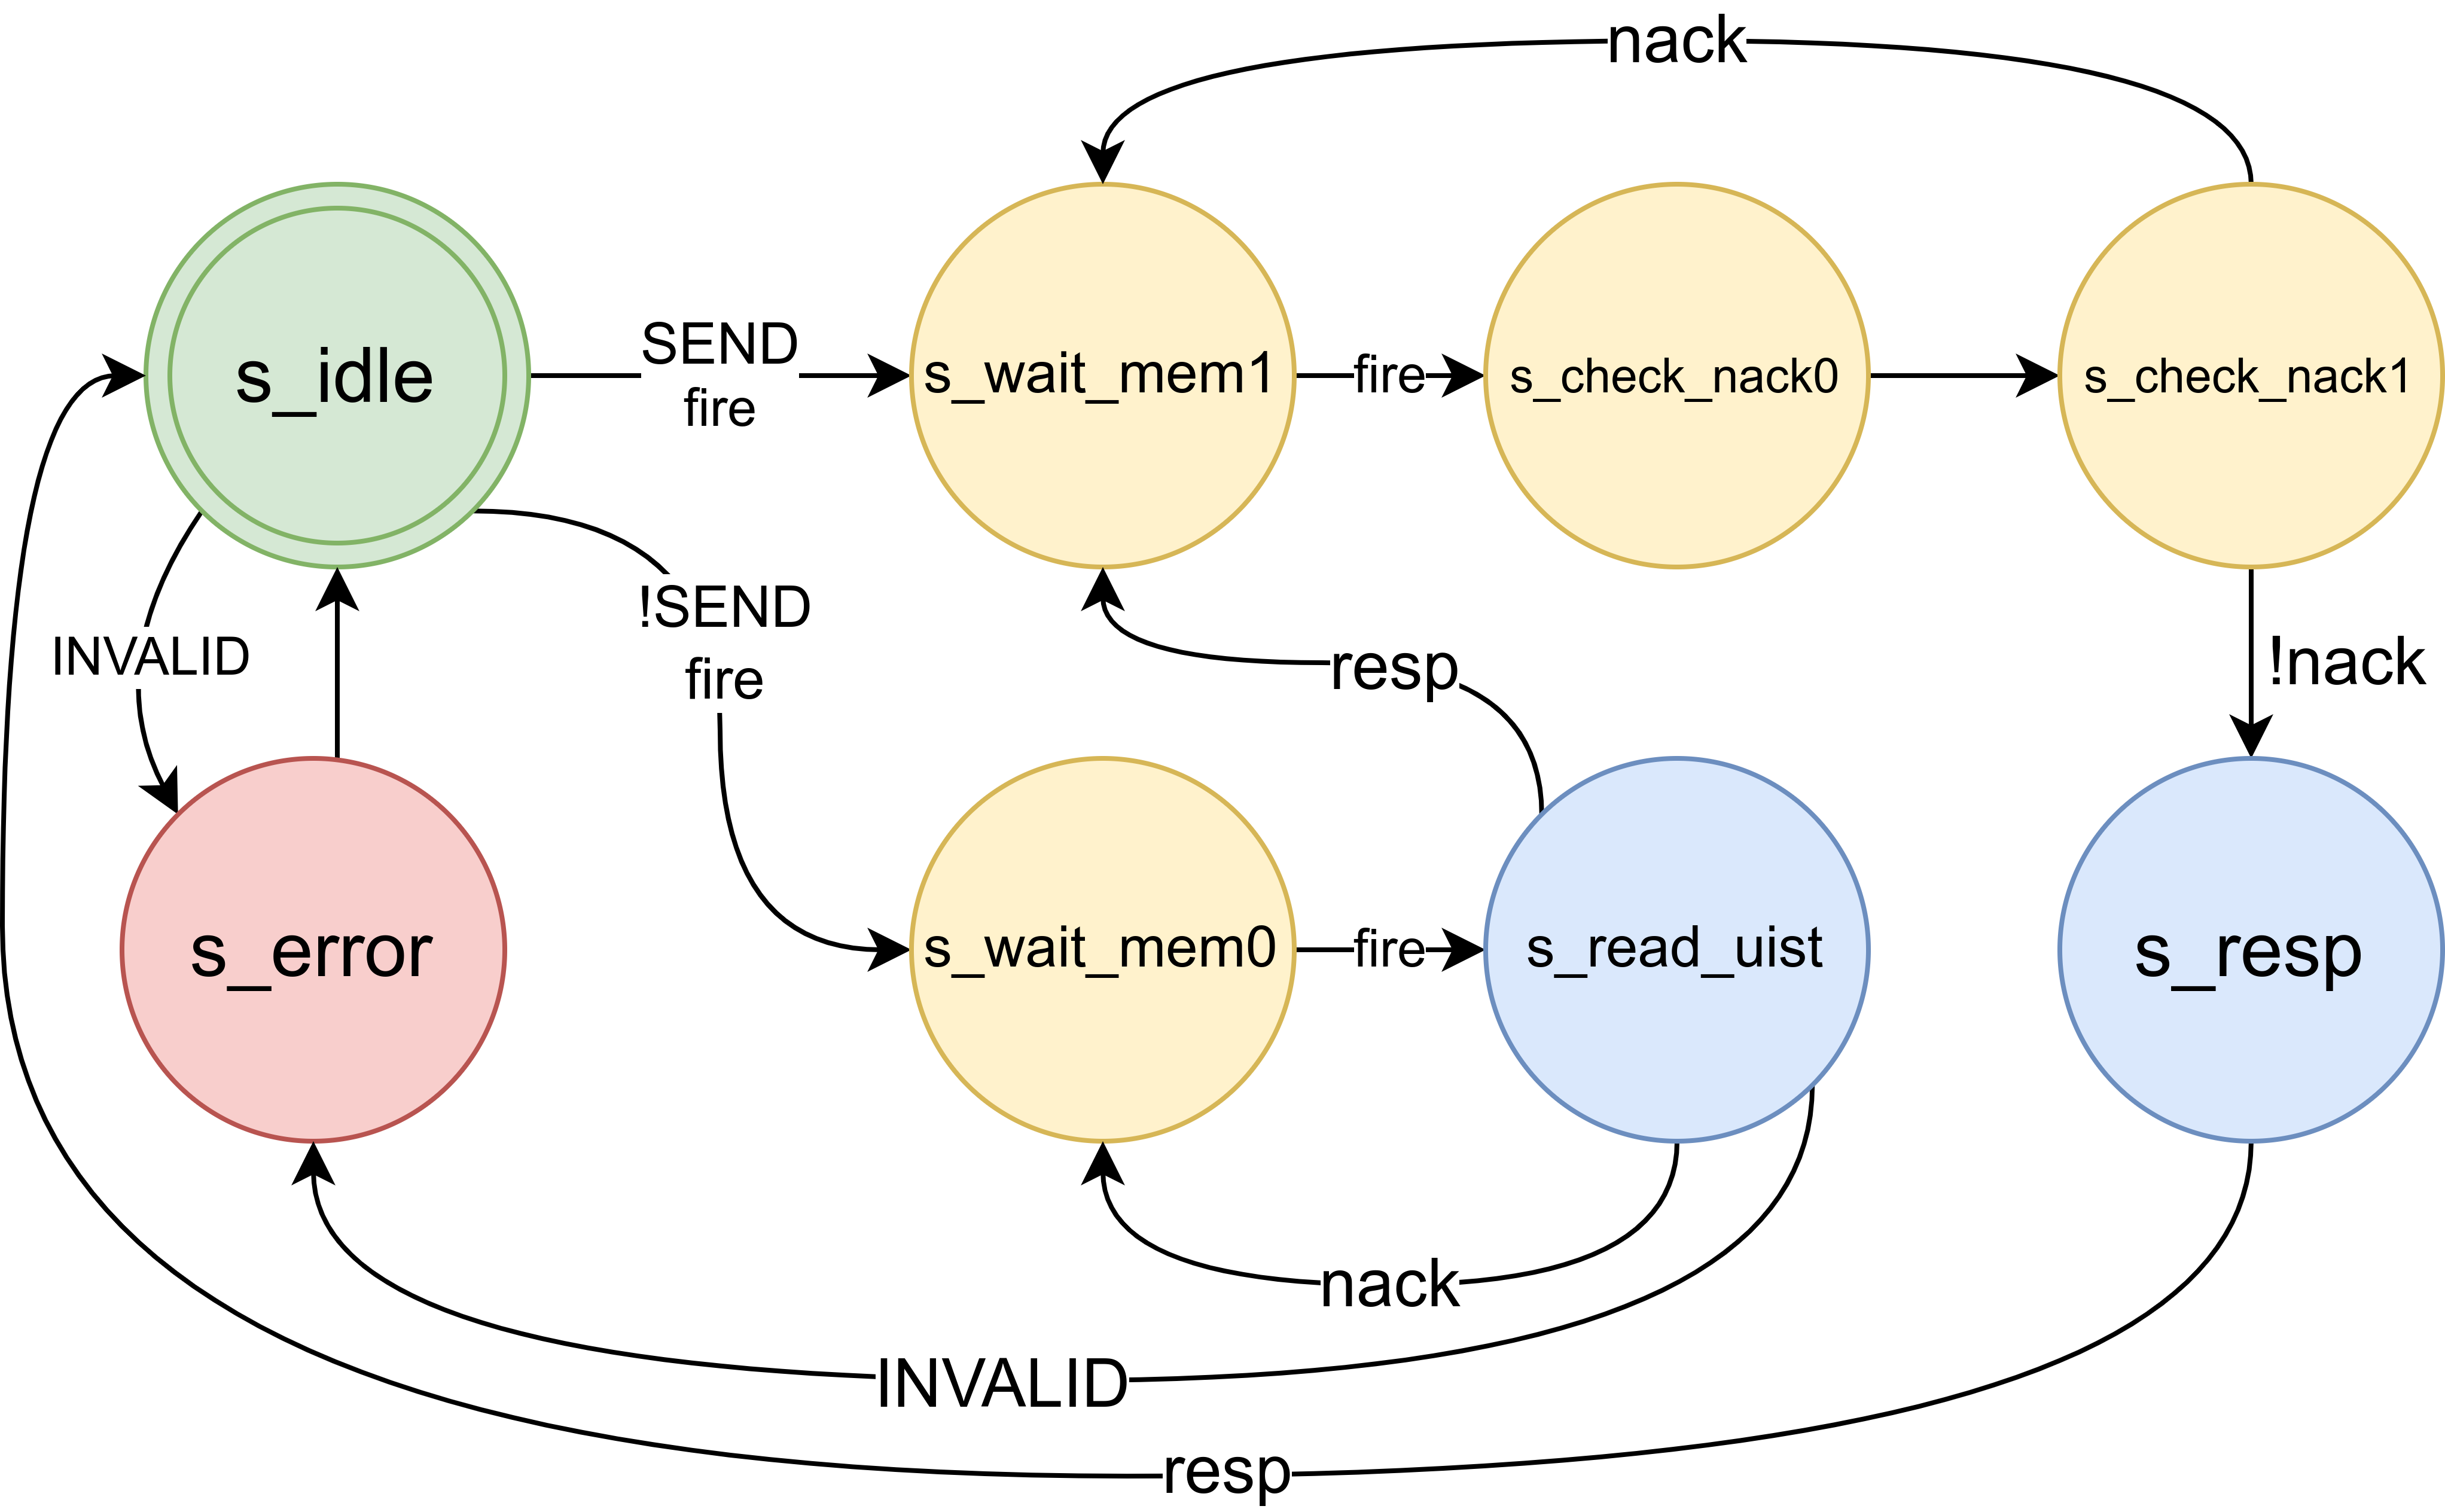
\includegraphics[width=1\linewidth]{figures/uipi.png}
    \caption{UIPI 协处理器工作流程}
    \label{fig:uintr3}
\end{figure}

UIPI 协处理器共发出三类访存请求:读内存,读外设,写外设,其中读内存请求可能因为数据缓存不命中需要重新发起请求,读写外设请求可能因为数据缓存事务繁忙需要重新发起请求,因此在处理流程中加入了对数据缓存 \texttt{s2\_nack} 信号的处理。此外,在 Rocket Chip 中存在一个缓存多个 RoCC 读写请求的队列模块,支持失败读写请求的重试,然而对于写外设请求,队列会持续等待响应信号并阻塞。因为目前只有一个 UIPI 协处理器,所以在架构中移除了这个模块并直接将 UIPI 协处理器连接到数据缓存的仲裁器。

\section{本章小结}

本章分两个层面介绍了硬件实现的方法,无论是在 QEMU 中还是在 Rocket Chip 中,改动都主要涉及三个方面,这三个方面分别对应设计方案的三部分内容,即 CPU 控制寄存器和状态维护,用户态中断控制器和 UIPI 指令。通过对 QEMU 的分析和改动,可以不断完善设计方案中的漏洞,最后将设计方案落实到真实的硬件中。Chisel 硬件描述语言强大的功能和丰富的抽象使得硬件逻辑更加清晰,帮助我们在开发过程中减少了使用传统硬件描述语言时遇到的各种错误。
% !TeX root = ret../thesis.tex

\chapter{软件实现}

\section{QEMU}

QEMU \cite{qemu} 为操作系统和用户态程序提供虚拟的执行环境,通过动态的二进制转换,模拟 CPU 的行为,同时支持多种外设的仿真,在系统开发中扮演着重要角色。
QEMU 支持模拟 RISC-V 运行环境,通过对 QEMU 的修改和测试,我们可以不断完善设计草案。对 QEMU 的修改主要分为四个方面:

\begin{itemize}
    \item 指令翻译:引入对 \Iuipi 指令的译码和执行;
    \item CPU 状态:维护 CSR 寄存器等 CPU 状态;
    \item 内存读写:\Iuipi 指令需要直接访问物理内存和 UINTC 外设,调用 \mintinline[breaklines]{C}{void cpu_physical_memory_rw(hwaddr addr, void *buf, hwaddr len, bool is_write)} 函数完成对物理地址的读写;
    \item 核间中断:实现 UINTC 并向各个核发送中断。
\end{itemize}

\subsection{指令翻译}

QEMU 翻译一条指令的过程为:从客户机指令(Guest Instructions)到中间码(TCG,Tiny Code Generator),最后再到宿主机指令(Host Instructions)。
QEMU 的翻译机制类似于 CPU 流水线中的译码阶段,需要定义模式串来帮助 QEMU 在执行到某一指令时调用对应的辅助函数。模式串的定义位于 target/riscv/insn32.decode :

\begin{lstlisting}
uipi_send       0000000  00000 ..... 010 ..... 1111011 @r2
uipi_read       0000001  00000 ..... 010 ..... 1111011 @r2
uipi_write      0000010  00000 ..... 010 ..... 1111011 @r2
uipi_activate   0000011  00000 ..... 010 ..... 1111011 @r2
uipi_deactivate 0000100  00000 ..... 010 ..... 1111011 @r2
\end{lstlisting}

以 \Iuret 这条指令为例,在 target/riscv/insn\_trans 目录下,有各种指令的翻译过程,主要用来将指令解析的结果(寄存器,立即数等)传递给辅助函数,将客户机指令拆解为宿主机指令来模拟目标指令的功能。
对于 \Iuret 指令的执行涉及到较多 CPU 状态的变化,会对 pc ,CSR 等产生影响, 辅助函数的定义位于 target/riscv/helper\.h,通过宏定义 DEF\_HELPER\_x 来声明辅助函数,例如:

\begin{lstlisting}[style=CStyle]
DEF_HELPER_1(uret, tl, env)
DEF_HELPER_4(csrrw, tl, env, int, tl, tl)
\end{lstlisting}

其中第一个参数对应辅助函数的名称 ,第二个参数代表函数的返回值类型(tl 表示 target\_ulong),后面的参数都是辅助函数传入的参数类型。有了以上的参考,我们可以定义其他辅助函数:

\begin{lstlisting}[style=CStyle]
DEF_HELPER_2(uipi_write, void, env, tl)
void helper_uipi_write(CPURISCVState *env, target_ulong src) {
    if (uipi_enabled(env, env->suirs)) {
        uint64_t addr = UINTC_REG_HIGH(env->suicfg, SUIRS_INDEX(env->suirs));
        cpu_physical_memory_write(addr, &src, 8);
    }
}
\end{lstlisting}

\subsection{CPU 状态}

CPU 状态的维护位于 target/riscv/cpu.h。这个结构同时考虑了 RV32、RV64、RV128 的情况,这些寄存器都是 CPU 运行时必要的状态。包括但不限于:

\begin{itemize}
    \item pc
    \item 整数、浮点寄存器堆
    \item CSR,有些寄存器是 M 态和 S 态复用的,例如 \Rmstatus、 \Rmip 等
    \item PMP 寄存器堆
    \item 通过 kernel\_addr、fdt\_addr 等从指定位置加载镜像
\end{itemize}

在target/riscv/cpu.h 文件末尾的表中注册 CSR 的操作函数。

中断异常、CSR 等宏定义位于 target/riscv/cpu\_bits.h ,我们需要在其中添加和 U 态有关的中断控制位。
CPU 中断异常处理函数位于 target/riscv/cpu\_helper.c 的最后,
这个函数对中断异常原因进行判断,并根据 CPU 当前的特权级做不同的处理。
这个函数只给出了 M 态和 S 态的中断异常处理,我们需要额外在此处加入委托给 U 态的中断异常处理,也就是读写 \Rustatus,\Rucause,\Ruepc 等寄存器。

\subsection{核间中断}

QEMU 支持对不同硬件环境的模拟,需要在 virt 硬件环境中添加 UINTC 外设的配置并生成设备树信息。

UINTC 代码实现位于 hw/intc/riscv\_uintc.c ,调用 riscv\_uintc\_realize 对 UINTC 进行初始化,将 UINTC 外设连接到总线上,并初始化总线地址空间。对外设中的状态寄存器(接收方状态寄存器,中断信号寄存器等)进行内存分配和初始化。
通过调用 qdev\_connect\_gpio\_out 默认将 UINTC 的中断信号绑定至每个核的 \Ruip 寄存器中的 \FcsrUipUsip 位。

\begin{lstlisting}[style=CStyle]
for (i = 0; i < num_harts; i++) {
    CPUState *cpu = qemu_get_cpu(hartid_base + i);
    RISCVCPU *rvcpu = RISCV_CPU(cpu);
    qdev_connect_gpio_out(dev, i, qdev_get_gpio_in(DEVICE(rvcpu), IRQ_U_SOFT));
}
\end{lstlisting}

最后完成对 UINTC 读写函数的注册,这样就可以直接通过物理地址访问 UINTC 外设的读写端口了:

\begin{lstlisting}[style=CStyle]
static const MemoryRegionOps riscv_uintc_ops = {
    .read = riscv_uintc_read,
    .write = riscv_uintc_write,
    .endianness = DEVICE_LITTLE_ENDIAN,
    .valid = {
        .min_access_size = 8,
        .max_access_size = 8
    }
};
\end{lstlisting}

在 UINTC 的实现中,中断是通过每次写入 UINTC 的端口来触发的,这和真实的硬件实现其实存在差异。
例如在 U 态,从目前的设计草案来看,需要同时满足以下几个条件才可以触发中断:

\begin{itemize}
    \item 当前特权级为 S 态
    \item \Rustatus 中 \FcsrUstatusUie 位是 1
    \item \Ruie 中 \FcsrUieUsie 位是 1
    \item \Ruip 中 \FcsrUipUsip 位是 1
\end{itemize}

在硬件实现中,可以看成是几个信号的与操作,当其他所有信号都拉高时,任何一个信号从低电平拉高都会触发中断,根据 RISC-V 的特权态规范\cite{rvpriv110},
\Isret 会将特权态从 S 态切换回 U 态,\Iuret 会将 \Rustatus 中的 \FcsrUstatusUie 位设置为 \FcsrUstatusUpie 位,在这两条指令后执行的第一条指令都有可能被中断打断并立刻进入中断处理的流程,
因此我们需要在 QEMU 中模拟这个过程,在 \Isret 和 \Iuret 指令中直接对上述条件进行判断和处理,例如在 \Isret 的辅助函数中:

\lstset{language=C}
\begin{lstlisting}[style=CStyle]
if (riscv_has_ext(env, RVN)
    && prev_priv == PRV_U
    && get_field(env->mip, MIP_USIP)
    && get_field(env->mstatus, MSTATUS_UIE)
    && get_field(env->sideleg, MIP_USIP)) {
    retpc = env->utvec;     // 直接跳转到U态中断处理入口
    env->uepc = env->sepc;  // 指定 \Iuret 到同一条指令
    mstatus = env->mstatus;
    mstatus = set_field(mstatus, MSTATUS_UPIE, 1);
    mstatus = set_field(mstatus, MSTATUS_UIE, 0);
    env->mstatus = mstatus;
}
\end{lstlisting}

\section{Linux}

Linux 是世界上最著名的开源操作系统。Linux 是标准的宏内核,可以在其上运行多种应用。目前 Linux 已经支持在 RISC-V 硬件平台上运行,也能在 QEMU 模拟的 RISC-V 硬件环境上运行。为了支持用户态中断并对其性能进行更深入的分析,我们对 Linux 6.0 版本进行了修改。针对 Linux 的修改主要分为三个部分:

\begin{itemize}
    \item 添加 UINTC 驱动并让 Linux 识别 UINTC 的设备树信息
    \item 接收方陷入内核前的状态的保存与恢复
    \item 注册并实现系统调用
\end{itemize}

\subsection{UINTC 驱动}

在 QEMU 的 virt 硬件环境中添加设备树生成代码,最后生成的设备树节点内容如下:

\lstset{basicstyle=\footnotesize\tt}
\begin{lstlisting}
uintc@2f10000 {
    interrupts-extended = <0x08 0x00 0x06 0x00 0x04 0x00 0x02 0x00>;
    reg = <0x00 0x2f10000 0x00 0x4000>;
    interrupt-controller;
    compatible = "riscv,uintc0";
};
\end{lstlisting}

其中各个字段的含义为:

\begin{itemize}
    \item \textbf{interrupts-extended} 连接到每个核 \Ruip 寄存器的 \FcsrUipUsip 位
    \item \textbf{interrupts-controller} 表示该设备是一个接收中断的控制器,这里加上是为了方便 Linux 识别,实际上 UINTC 并没有接收外部中断
    \item \textbf{compatible} 表示设备名称,Linux 内注册驱动时应该与之对应
\end{itemize}

驱动代码位于 drivers/irqchip/irq-riscv-uintc.c ,Linux 对 UINTC 进行的初始化过程如下:

\begin{itemize}
    \item 解析设备树获取外设对应的物理地址范围
    \item 初始化全局控制结构 \ref{code:uintcpriv} 并保存外设信息
    \item 调用 \mintinline[breaklines]{c}{void __iomem *ioremap(phys_addr_t addr, size_t size)} 完成内核物理地址到虚拟地址的映射,内核可以通过虚拟地址直接访问 UINTC 读写端口
    \item 初始化全局位图管理 UINTC 中已分配的槽位
\end{itemize}

\label{code:uintcpriv}
\begin{lstlisting}[style=CStyle]
    struct uintc_priv {
        struct cpumask lmask; // 位图记录已连接的 CPU
        void __iomem *regs;   // UINTC 在内核地址空间映射的起始地址
        resource_size_t size; // UINTC 地址范围大小
        u32 nr;               // UINTC 槽位数量
        void *mask;           // 位图记录已分配的槽位
        spinlock_t lock;      // 互斥锁
    };
\end{lstlisting}

\subsection{状态保存与恢复}

arch/riscv/kernel/entry.S 是 Linux 在 RISC-V 硬件平台上运行时的陷入入口,涉及上下文的保存与恢复、针对不同陷入原因跳转到对应的处理函数入口、针对不同系统调用号跳转到系统调用向量表对应的入口等。

Linux 中线程也被称为轻量级进程(LWP, Light-weight process)\cite{linuxbook},如无特殊说明,描述中默认使用进程指代进程或线程。考虑到在某些负载环境下,接收方进程可能在不同核上迁移,需要对用户态的控制状态进行保存与恢复,主要对 \Rutvec 、\Ruscratch、\Ruepc 三个寄存器进行保存。此外还需要在陷入时将接收方状态的 Active 位置 0 确保当这个核运行其他进程时不会被中断。接收方被唤醒并准备在某个核上运行前,除了对上述三个寄存器进行恢复外,还需要设置 \Rsuirs 寄存器,注意到当进程主动让权时,内核会两次进入 resume\_userspace 这个代码段,因此只能在 restore\_all 这个代码段重新将接收方状态的 Active 位置 1 确保被唤醒的是真正运行在这个核上的进程。

\subsection{进程管理}

在 arch/riscv/kernel/uintr.c 中添加用户态中断相关代码,主要涉及以下内容:

\begin{itemize}
    \item 控制结构定义和初始化:在进程控制块中维护发送方和接收方的状态
    \item 进程资源分配和回收:文件描述符,进程控制块内的状态,发送方状态表等
    \item 系统调用实现:在系统调用向量表中注册系统调用号,并通过 SYSCALL\_DEFINEx 宏声明并实现系统调用函数
\end{itemize}

\section{libc}

\subsection{API 实现}

对系统调用进一步封装,包括设置 U 态 CSR 、上下文保存与恢复以及读取并更新 UINTC 中的 Pending Requests 等:

\begin{lstlisting}[style=CStyle]
    #include "uintr.h"

    extern void __handler_entry(struct __uintr_frame* frame, void* handler) {
        uint64_t irqs = uipi_read();
        csr_clear(CSR_UIP, MIE_USIE);
        uint64_t (*__handler)(struct __uintr_frame * frame, uint64_t) = handler;
        irqs = __handler(frame, irqs);
        uipi_write(irqs);
    }
    static uint64_t __register_receiver(void* handler) {
        // 设置中断处理函数入口
        csr_write(CSR_UTVEC, uintrvec);
        csr_write(CSR_USCRATCH, handler);
        // 使能 U 态中断处理
        csr_set(CSR_USTATUS, USTATUS_UIE);
        csr_set(CSR_UIE, MIE_USIE);
        int ret = __syscall0(__NR_uintr_register_receiver);
        // 使能 UINTC 
        uipi_activate();
        return ret;
    }
    // 用户调用接口
    #define uintr_register_receiver(handler) __register_receiver(handler)
\end{lstlisting}

注意到上述代码并没将用户注册的函数直接赋值给 \Rutvec 寄存器,而是赋值给了 \Ruscratch ,这是因为在汇编代码中需要先将通用寄存器保存在栈上,然后才能开始执行用户注册的函数。

\subsection{APP 示例}

根据图 \ref{fig:uintr2} 中 RISC-V 用户态中断的工作流程,可以实现一个简单的进程间通信应用。

\begin{lstlisting}[style=CStyle]
    volatile unsigned int uintr_received; // volatile 避免编译优化
    unsigned int uintr_fd;

    uint64_t uintr_handler(struct __uintr_frame *ui_frame, uint64_t irqs) {
        uintr_received = 1; // 设置标志位
        return 0;
    }

    void *sender_thread(void *arg) {
        int uipi_index;
        // 注册发送方状态表项
        uipi_index = uintr_register_sender(uintr_fd);
        // 发送用户态中断
        uipi_send(uipi_index);
        return NULL;
    }

    int main() {
        pthread_t pt;
        int ret;
        // 注册接收方中断处理函数
        if (uintr_register_receiver(uintr_handler))
            exit(EXIT_FAILURE);
        // 注册文件描述符
        ret = uintr_create_fd(1);
        if (ret < 0) exit(EXIT_FAILURE);
        uintr_fd = ret;
        // 创建发送方
        if (pthread_create(&pt, NULL, &sender_thread, NULL))
            exit(EXIT_FAILURE);
        // 忙等待标志位
        while (!uintr_received);
        pthread_join(pt, NULL);
        close(uintr_fd);
        // 正常退出
        exit(EXIT_SUCCESS);
    }
\end{lstlisting}

接收方注册中断处理函数,注册文件描述符,创建发送方进程,并忙等待标志位;发送方进程注册后发送一个中断便直接退出;接收方收到中断并陷入中断处理函数后设置标志位,回到正常流程发现标志位已被设置,继续执行直到退出。
% !TeX root = ../thesis.tex

\chapter{系统评估}

本章重点介绍在 FPGA 上对系统的构建和评估,实验的目标主要分为以下几个方面:

\begin{itemize}
    \item 验证硬件实现的正确性;
    \item 验证软件实现的正确性;
    \item 验证软硬件协同设计的用户态中断的性能优势;
    \item 分析测试结果与硬件行为间的联系。
\end{itemize}

\section{实验环境}

\begin{figure}
    \centering
    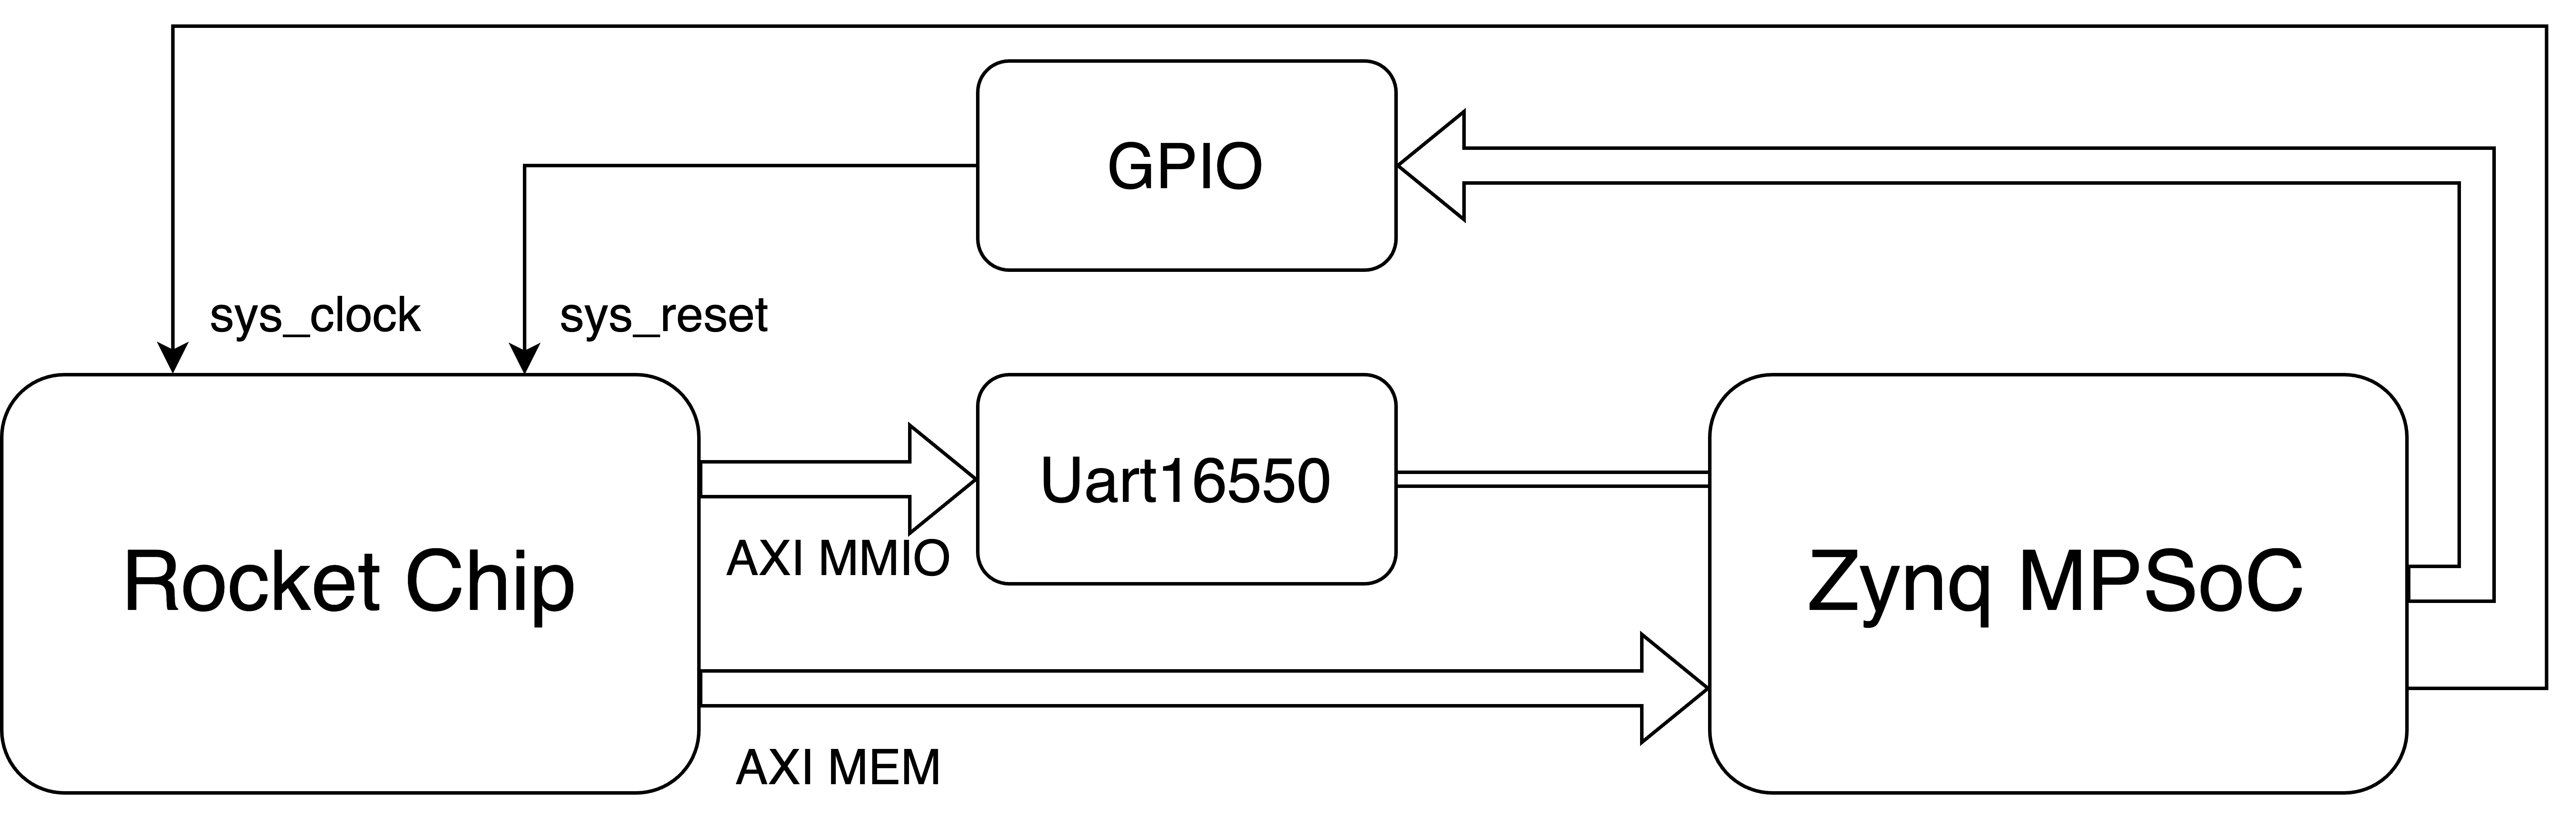
\includegraphics[width=0.8\linewidth]{figures/soc.png}
    \caption{SoC 整体架构}
    \label{fig:soc}
\end{figure}

本文实验主要在 Zynq UltraScale+ MPSoC ZCU102 开发板上开展。ZCU102 分为两个部分,分别为处理器子系统(PS) 和 可编程逻辑(PL) 。PS 提供一款四核 ARM® Cortex®-A53、双核 Cortex-R5F 实时处理器,可以直接对开发板上的资源进行控制;PL 端可以通过 DDR4 组件访问内存资源。

首先,应用 Xilinx 提供的 petalinux SDK 构建在 PS 上运行的 Linux 系统,并挂载 SD 卡作为系统的存储外设。如图 \ref{fig:soc} 所示,引入 AXI GPIO IP 核并在 PS 的设备树给出相关信息,GPIO 的出端口连接到 Rocket Chip 内部,可以在 PS 上操作 /sys/class/gpio/* 来写入这个端口对 Rocket Chip 进行复位。

利用 Rocket Chip 支持的自定义端口和自定义配置参数构建顶层模块。自定义配置包括加入第三章最后一节介绍的 UIPI 协处理器,设置 BootROM 的地址和加载内容。Rocket Chip 顶层模块需要对外暴露两个 AXI master 接口,MEM 端口访问位于 PS 端的 DDR 控制器,MMIO 端口访问 PL 上引入的 Uart16550 IP 核。关于两个端口的地址映射,需要将 Rocket Chip 配置的映射和 Block Design 构建时指定的地址映射相对应。

进一步地,定义系统的顶层模块对 Rocket Chip 顶层模块和 Block Design 模块进一步封装,该模块会对 AXI 接口的位宽进行处理,此外,由于 Rocket Chip 默认看到的内存起始地址为 0x80000000 ,而 Block Deisgn 中 DDR 控制器访问端口的地址映射起始地址为 0 ,需要在模块中对地址高位进行截断。

为了与 Rocket Chip 上运行的系统软件进行交互,引入 Uart16550 IP 核,虽然 Rocket Chip 能够自动生成与内部配置有关的设备树信息,但缺少 PL 额外引入的设备的设备信息,需要手动加入 Uart16550 的设备树节点。

\begin{figure}
    \centering
    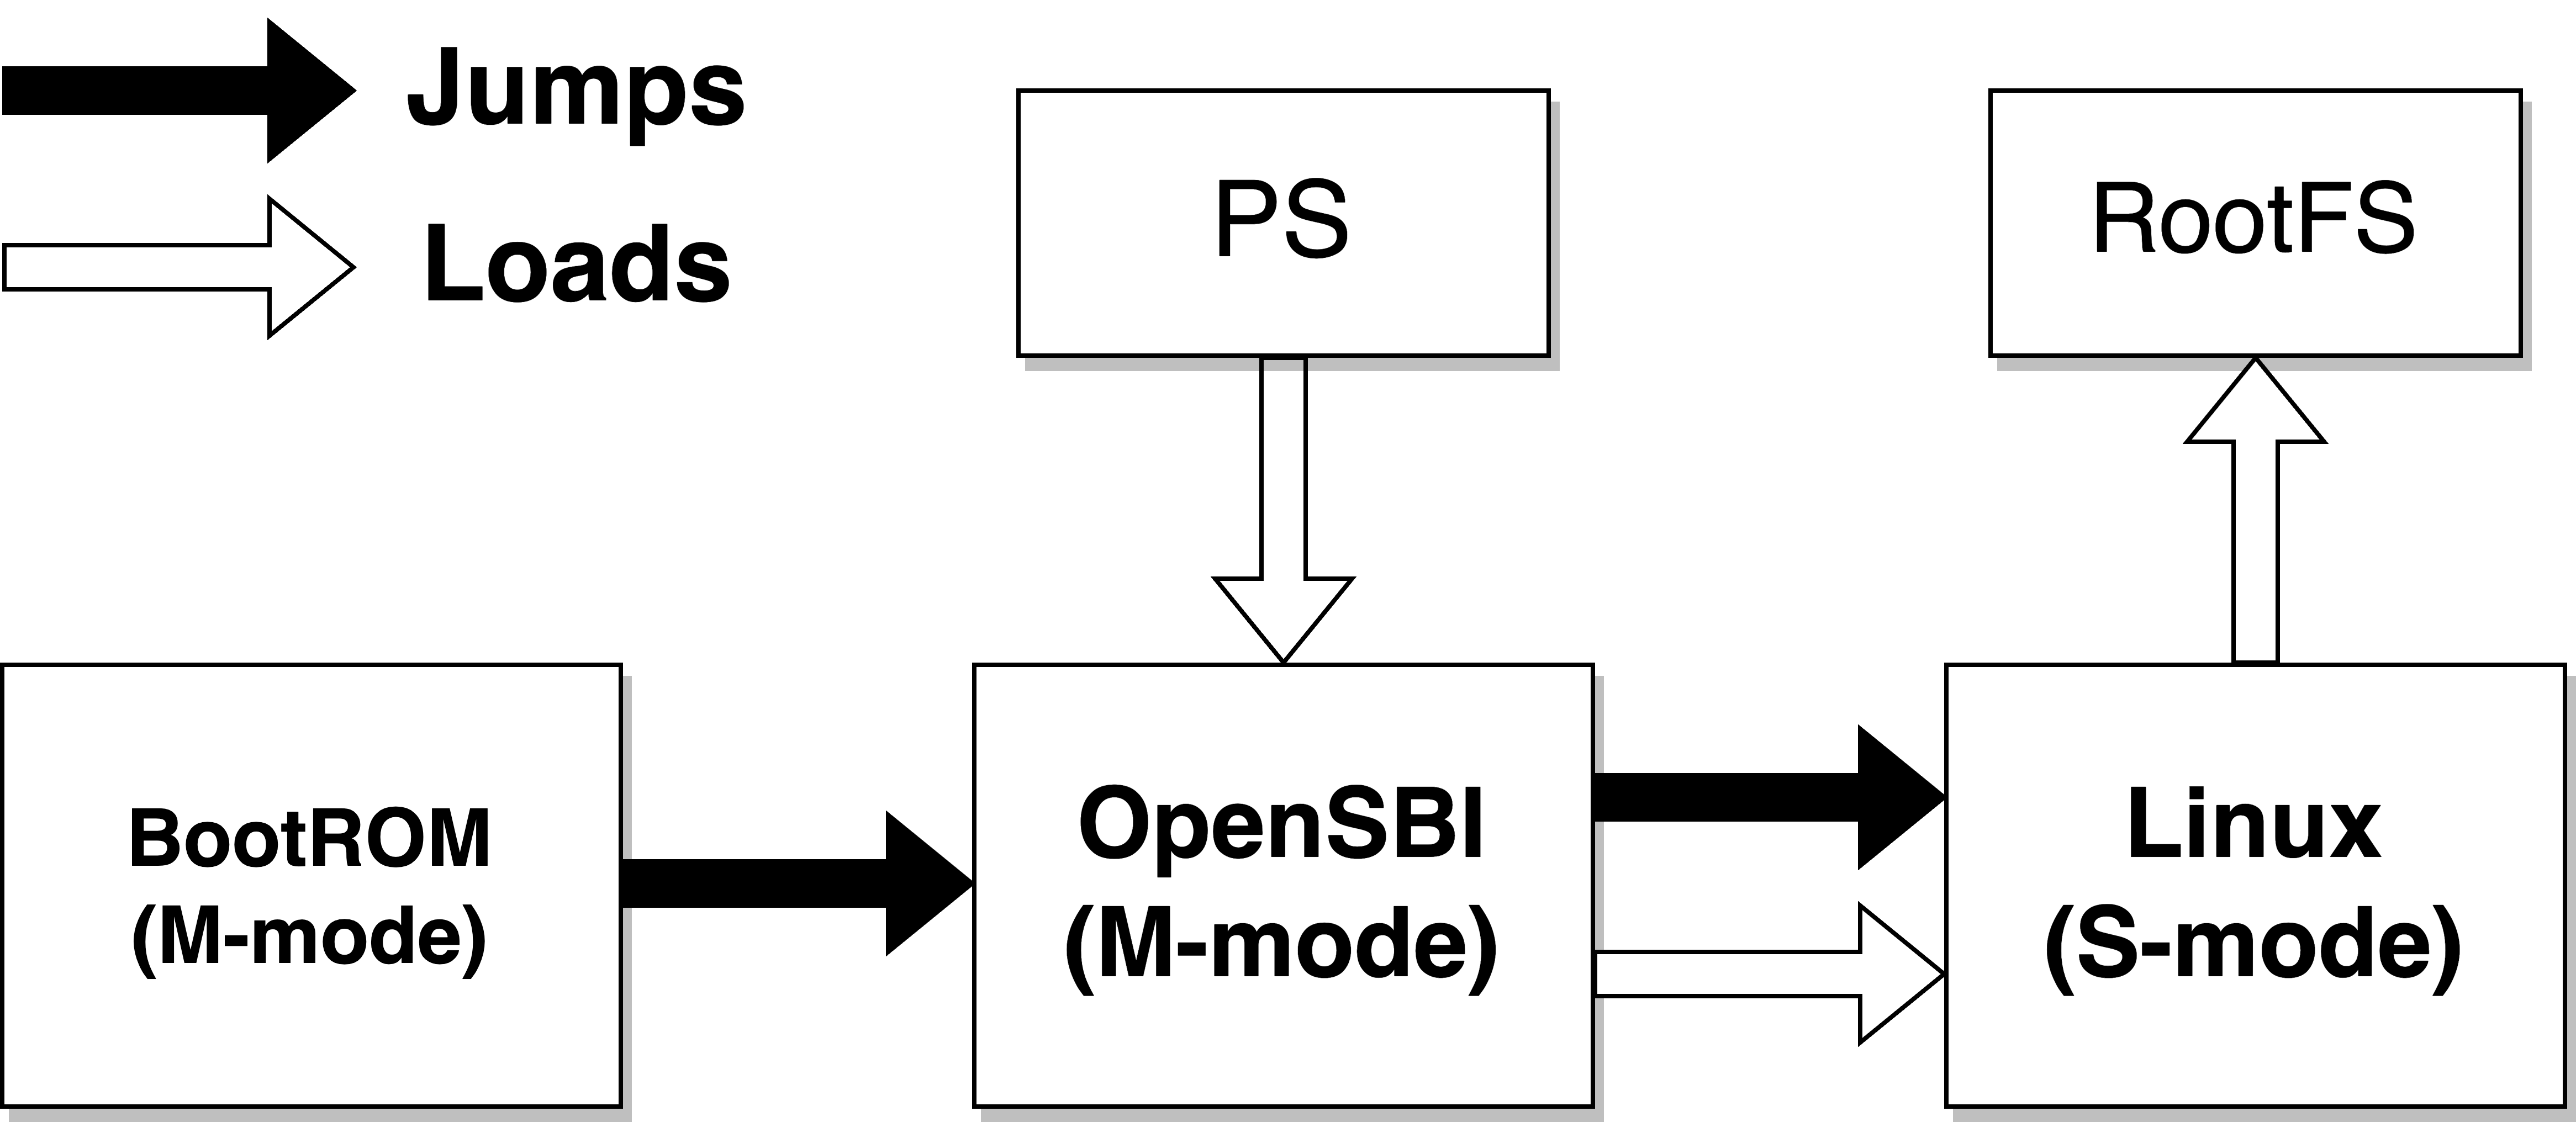
\includegraphics[width=0.8\linewidth]{figures/boot.png}
    \caption{系统软件启动流程}
    \label{fig:boot}
\end{figure}

系统软件的启动流程如图 \ref{fig:boot} 所示。BootROM 为 Rocket Chip 内置的启动代码,在构建时会提前写入到模块中,跳转地址默认为内存的起始地址。

OpenSBI (RISC-V Open Source Supervisor Binary Interface) \cite{opensbi} 是 RISC-V 架构下的 Bootloader,支持通用 SBI 接口,支持 dynamic、jump、payload 三种启动方式。本文的实验采用 payload 启动方式,OpenSBI 镜像会根据 Linux 镜像和设备树的文件位置一起构建。OpenSBI 会在运行时将 Linux 镜像加载到目标地址,并将设备树放在指定的地址。跳转到 Linux 镜像前,OpenSBI 会将核号、设备树地址等信息传递给 Linux 用于 Linux 进一步的初始化。

Buildroot \cite{buildroot} 是一个构建嵌入式 Linux 系统的框架。本文的实验使用 Buildroot 构建根文件系统,并在 Linux 的编译选项中指定文件系统镜像的位置,让 Linux 镜像与文件系统镜像一起构建,并将该文件系统作为 initramfs 。此外,为了让 Linux 在启动时可以打印日志,需要在设备树中添加启动参数指定 earlycons 。

如前文所述,PS 可以对 Rocket Chip 进行复位,在复位前,需要把构建好的 OpenSBI 镜像拷贝到内存中,这部分内存以 reserved-memory 的形式挂载到 PS 的 /dev/mem 文件上,PS 可以直接对该文件进行 mmap 操作完成镜像的写入。

Linux 启动后,可以在主机上连接开发板的串口并看到输出:

\begin{figure}
    \centering
    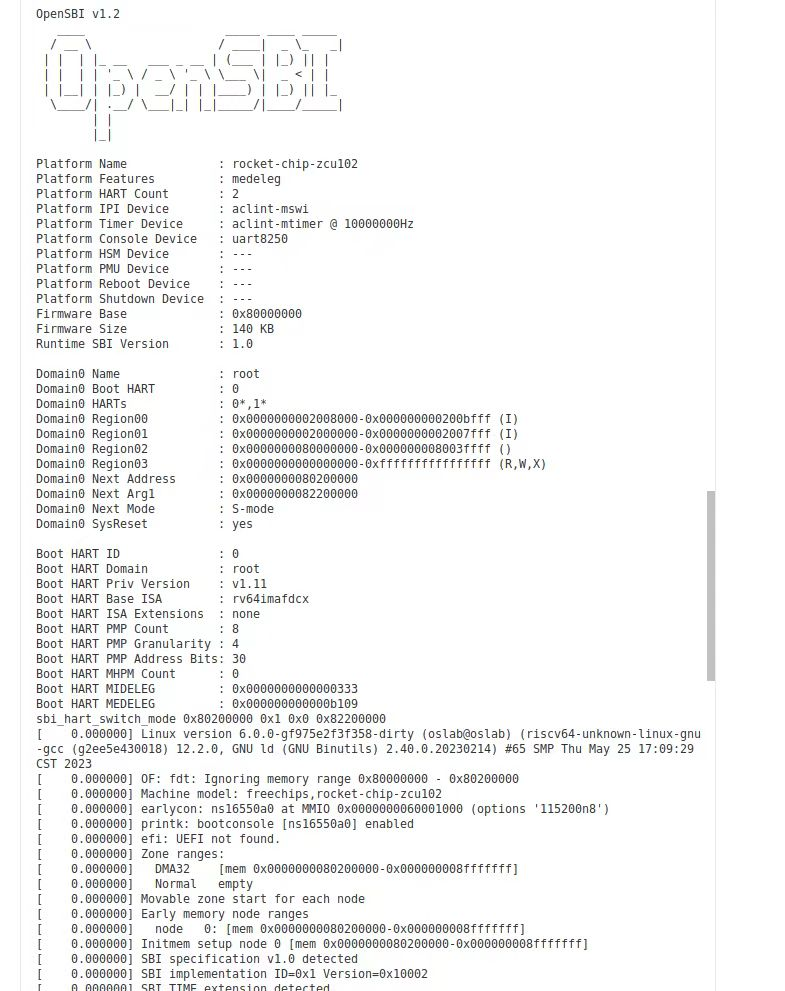
\includegraphics[width=0.9\linewidth]{figures/boot-linux.jpg}
    \caption{启动 Linux}
    \label{fig:boot-linux}
\end{figure}

\section{功能测试}

\subsection{Verilator 仿真测试}

Verilator \cite{verilator} 是一款开源的硬件描述语言仿真器,可以生成 C++仿真代码并在主机上模拟硬件电路的行为。相比于传统的基于事件的仿真器,Verilator 可以更快速、准确地模拟大型电路。
Rocket Chip 集成了 Verilator 仿真器,可以在综合前对 Rocket Chip 进行行为仿真,通过观察 Verilator 生成的波形,可以提早发现并解决硬件逻辑问题,减少硬件调试带来的开销。

riscv-tests \cite{riscvtests} 是一个开源的验证 RISC-V 处理器正确性的测试集,由 RISC-V 基金会开发和维护,包括了 RISC-V 指令集的大部分指令和特性的测试。Rocket Chip 集成该项目并利用 Verilator 对这些测例进行仿真。
基于这一项目,我们实现了多个针对 RISC-V 用户态中断的测例,覆盖了读写 CSR 、中断处理、UIPI 指令等特性。

\subsection{软件接口测试}

\begin{figure}
    \centering
    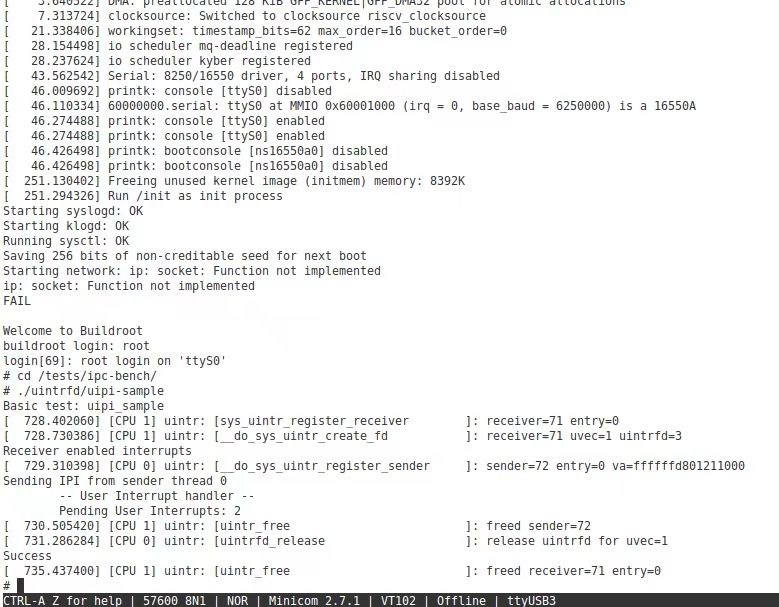
\includegraphics[width=0.8\linewidth]{figures/uipi-sample.jpg}
    \caption{应用程序输出}
    \label{fig:uipi-sample}
\end{figure}

在第四章最后一节中,我们介绍了一个简单的用户态进程间通信程序。分别在 QEMU 模拟器和 Rocket Chip 上启动修改后的 Linux 并运行该程序,可以看到发送方和接收方均正常退出,并释放占用的内核资源,包括文件描述符、发送方状态表等。

\section{性能测试}

ipc-bench \cite{ipcbench} 是一个用来的测试 Linux 和 OS X 操作系统上 IPC 性能的开源项目,包括信号、管道、FIFO、共享内存、TCP 等 IPC 机制。为减少用户程序层面的干扰,对于不同的 IPC 机制采用相同的 Ping-Pong 通信模型,通信的双方会忙等待对方的消息。每个测例会根据配置参数决定某一方收或发的总次数和消息的大小,执行结束后在命令行打印计算得到的性能指标,包括通信的总时间,平均每次通信的时间,吞吐量,标准差。但是实际在统计测试结果时,我们并未完全采纳输出的信息,后续会给出具体的分析。

基于第四章第二节中的库函数,利用 ipc-bench 项目提供的环境,我们实现了针对用户态中断的测试程序。为满足 Ping-Pong 通信模型,该测试程序的通信两端需要同时作为接收方和发送方。在通信开始前,两个线程需要进行一系列的配置,这部分配置不会被包含在总通信时间中。正如上一节所介绍的,我们运行测试的硬件环境是 Rocket Chip,ipc-bench 项目在统计通信时间时,还统计了每次通信的时间来分析标准差等性能指标,需要在每次通信时调用 \texttt{timespec\_get} 函数。这个函数会执行系统调用陷入内核,内核为了获取硬件寄存器中包含的时间信息,执行了 \texttt{rdtime} 这条伪指令,会进一步陷入 OpenSBI 中读取 CLINT 硬件寄存器,整个流程涉及大量的上下文切换,成为了实际的性能瓶颈。对于信号和管道等测例来说可能影响并不是很显著,但是对于 eventfd 和用户态中断等机制来说,每次通信都获取时间会降低测试的准确性。因此在后续的测试中,除用户态中断的测试程序以外,我们也修改了性能对比中用到的测试程序,包括信号、管道和 eventfd ,具体的修改方案为移除每次通信的时间统计,只在通信循环的开始和结束获取时间并计算出通信的总时间。此外,在用户态中断中,消息的大小恒为 1 bit,因此在运行其他测例时,也指定消息大小为 1 bit。

\section{测试结果与分析}

如图是用户态与不同 IPC 机制的性能对比结果。

总体上来看,用户态中断的性能明显优于其他 IPC 机制,说明用户态中断从发出到响应的延迟很低;具体到指令周期,通过 ILA 抓取 Rocket Chip 中的 \texttt{pc} 寄存器,从发送方所在的核执行 \Iuipisend 这条指令开始,到接收方所在的核触发中断处理流程,\texttt{pc} 跳转到 \Rutvec ,总共需要约 100 个时钟周期;根据第四章第二节中对于库函数的介绍,在执行用户指定的中断处理函数之前,需要进行通用寄存器的保存,大概需要约 400 个时钟周期。也就是说从发送方发送用户态中断到接收方响应并开始处理共需要约 500 个时钟周期,这已经远小于应用程序陷入内核再返回的开销了。

相比于其他的 IPC 机制,用户态中断的性能存在一定的波动。在进行软件适配时,需要考虑到接收方是否正在某个核上运行,理想情况下是接收方一直在某个核上运行,用户态中断的延迟可以达到上述的指令周期数;当目标核正处于内核态或运行其他进程时,只有 UINTC 的 Pending Requests 位被写入,UINTC 不会触发用户态中断。当目标接收方被调度时,内核才会在返回用户态前将当前核号写入 UINTC 并将 Active 位置为 1,从而在执行 \Isret 返回用户态的第一条指令触发用户态中断并陷入到用户态中断处理函数中。接收方不在核上运行的流程可以类比用户为某个信号注册处理函数的情况,二者都是经历了\textbf{恢复-陷入-恢复} 的过程,在这种情况下,用户态中断的响应延迟会增加,但一般来说会比信号的处理更快,因为信号处理需要两次切换特权级,而用户态中断只需要一次切换特权级,所以用户态中断的处理相比信号的处理对于页表和缓存系统来说更加友好。时钟中断会导致用户程序陷入到内核,从而导致用户态中断的响应延迟增加,因此用户态中断性能存在一定波动。

在实验的设计中,我们尽可能地减少其他因素对结果的影响,可以将通信总时间与通信次数近似地看成线性关系,从而可以计算出回归方程,其中斜率为单次通信的时间,因为实验开始时要获取时间,且缓存系统也需要预热,所以截距不为 0 。对比单次通信的时间,可以计算出用户态中断相对于其他 IPC 机制的加速比:


% !TeX root = ../thesis.tex

\chapter{结论}

本文提出了 RISC-V 用户态中断扩展方案,并通过软硬件协同的方式,对设计方案进行了验证和测试。实验结果表明,在本文搭建的测试环境中,用户态中断相比于信号机制,可以取得 203 倍的性能提升;相比于 eventfd,可以取得 136 倍的性能提升。

本文的工作聚焦于用户态中断扩展方案的设计与实现,重点对用户态中断的性能进行评估。在未来的工作中,可以更多地探索用户态中断的异步机制,并通过更复杂的应用场景如微内核等来发挥用户态中断的优势。

% 其他部分
\backmatter

% 参考文献
\bibliography{ref/refs}  % 参考文献使用 BibTeX 编译
% \printbibliography       % 参考文献使用 BibLaTeX 编译

% 致谢
% !TeX root = ../thuthesis-example.tex

\begin{acknowledgements}
  衷心感谢导师×××教授和物理系××副教授对本人的精心指导。他们的言传身教将使我终生受益。

  在美国麻省理工学院化学系进行九个月的合作研究期间,承蒙 Robert Field 教授热心指导与帮助,不胜感激。

  感谢×××××实验室主任×××教授,以及实验室全体老师和同窗们学的热情帮助和支持!

  本课题承蒙国家自然科学基金资助,特此致谢。
\end{acknowledgements}


% 声明
\statement
% 将签字扫描后的声明文件 scan-statement.pdf 替换原始页面
% \statement[file=scan-statement.pdf]
% 本科生编译生成的声明页默认不加页脚,插入扫描版时再补上;
% 研究生编译生成时有页眉页脚,插入扫描版时不再重复。
% 也可以手动控制是否加页眉页脚
% \statement[page-style=empty]
% \statement[file=scan-statement.pdf, page-style=plain]

% 附录
% 本科生需要将附录放到声明之后,个人简历之前
\appendix
% !TeX root = ../thesis.tex

\begin{translation}
\label{cha:translation}

\title{RISC-V 高级中断架构(第一章至第三章)}
\maketitle

\tableofcontents

\section{引言}

这篇文档给出了 RISC-V 高级中断架构的规范,包括:

\begin{itemize}
    \item[(a)] 针对 RISC-V 特权架构规范的扩展;
    \item[(b)] 两个标准的 RISC-V 中断控制器:高级平台级中断控制器(APLIC)和
\end{itemize}

\subsection{目标}
\subsection{限制}

\end{translation}


% TODO
% 本科生的综合论文训练记录表(扫描版)
% \record{file=scan-record.pdf}

\end{document}
